\chapter{Conclusioni}
Dai risultati raccolti e presentati nel precedente capitolo è evidente la differenza di accuratezza raggiunta sui due dataset. In particolare, nonostante si riesca facilmente ad ottenere un modello con risultati buoni o ottimi sul dataset WESAD, ciò non è stato ottenuto sul dataset ASCERTAIN originale mentre si hanno risultati sensibilmente migliori sullo stesso dataset ASCERTAIN modificato rendendo ogni soggetto più bilanciato riguardo le classi contenute.

% traccia possibile \/
% differenza wesad -- ascertain -> cosa rende risultati su wesad così migliori?
% importanza del bilanciamento dei dati
% approcci continui ottimi a seconda dei dati
% approcci che allo stato attuale sembrano funzionare meglio rispetto alla tipologia di dati
% applicabilità future a seconda dei dati disponibili

\section{Differenze fra i due dataset}
Uno degli elementi da considerare quando si addestra una rete neurale è il bilanciamento dei dati presi in considerazione per l'addestramento.\\
Andando ad analizzare nel dettaglio la struttura dei due dataset considerati, diventa evidente la decisa sovrarappresentanza della classe 0 nel dataset ASCERTAIN, mentre le classi nel dataset WESAD risultano molto più bilanciate. Questo è anche dovuto all'aver scelto delle classi fittizie, per quanto riguarda ASCERTAIN, che ha evidenziato come non tutti i soggetti abbiano prodotto dati bilanciati rispetto alle nuove classi selezionate.\\\\
Bilanciando il dataset ASCERTAIN attraverso la produzione di soggetti fittizi, ognuno contenente dati presi da tutti i soggetti in maniera bilanciata rispetto alle nuove classi, otteniamo immediatamente risultati sensibilmente migliori, con accuratezze a volte anche doppie rispetto allo stesso approccio sul dataset ASCERTAIN originale. Questo rende evidente l'importanza dell'avere dati di addestramento bilanciati, quindi esempi in quantità simile per ognuna delle etichette possibili.
\begin{figure}[h]
    \begin{minipage}[b]{0.5\textwidth}
		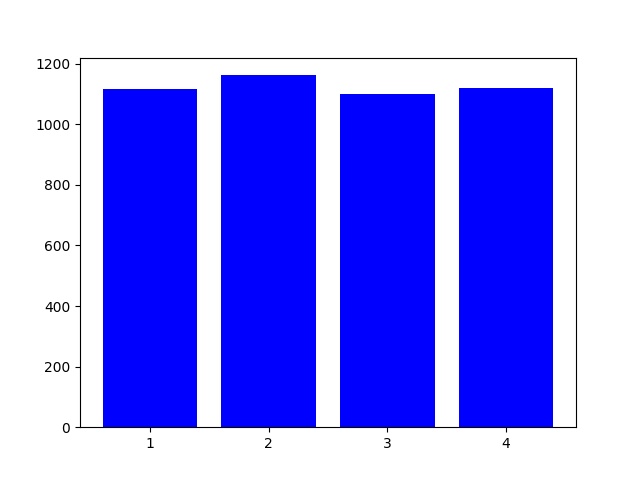
\includegraphics[width=\textwidth]{img/graphs/wesad_dataset.png}
		\caption{Presenza delle classi su dataset WESAD}
		\label{fig:wesadclasses}
	\end{minipage}
    \hfill
    \begin{minipage}[b]{0.5\textwidth}
		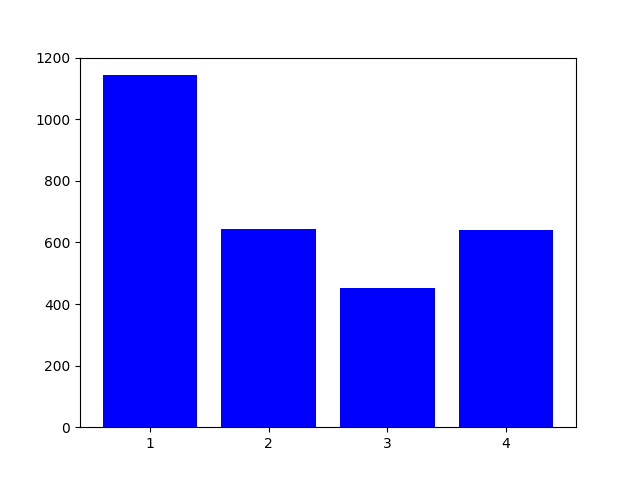
\includegraphics[width=\textwidth]{img/graphs/ascertain_dataset.png}
		\caption{Presenza delle classi su dataset ASCERTAIN}
		\label{fig:ascertainclasses}
	\end{minipage}
\end{figure}

\section{Approcci continual vs offline}
In tutti i dataset, gli approcci continui hanno mostrato accuratezza media inferiore rispetto all'addestramento offline: sul dataset WESAD si ha una riduzione dell'accuratezza media del 23.17\% in media sui vari approcci, mentre sul dataset ASCERTAIN si attesta sul 5.02\%. Su ASCERTAIN modificato rendendo ogni soggetto più bilanciato, invece, la riduzione media è dell'1.39\%, con la maggior parte degli approcci che ottengono un'accuratezza inferiore di meno dell'1\%.\\
Questa riduzione dell'accuratezza è sicuramente mitigabile attraverso la selezione di un modello con performance migliori negli approcci continui, invece di eseguire la \textit{model selection} sulla base dei risultati ottenuti nell'approccio offline. Con questi dati però si può già affermare che nella maggior parte dei casi gli approcci continui sono paragonabili all'addestramento classico, posto di avere un dataset con determinate caratteristiche: le classi all'interno del dataset di addestramento devono essere bilanciate fra loro, o si avrà un aumento di difficoltà nell'addestramento della rete neurale.\\\\
Si può quindi concludere che su certe tipologie di dati, il continual learning è applicabile all'ambito dello \textit{human state monitoring} con un elevato grado di accuratezza e ottenendo modelli di machine learning in grado di ottenere risultati comparabili o simili all'approccio offline. Il risultato più vicino all'addestramento offline è stato ottenuto con l'approccio cumulativo su dataset WESAD, con il replay al 25\% sul dataset ASCERTAIN e di nuovo con l'addestramento cumulativo sul dataset ASCERTAIN con i soggetti bilanciati artificialmente. Questo dimostra che mantenere esempi precedenti porta ad un addestramento di maggior qualità e un modello più capace di inferire correttamente lo stato psico-fisico di una persona, posto di avere sufficiente memoria per lo stoccaggio dei dati di replay.